\chapter{Uncertainties in the cross section measurement}\label{chap:Unc}
\minitoc
The cross section measurement relies on theoretical models and corrections, used in the Monte Carlo. Thus, their intrinsic uncertainties should be propagated to a final result. This chapter discusses main methods of uncertainties measurements. The sources of systematic uncertainties on $C_{W/Z}$ are discussed in Sec.~\ref{sec:cwErr}, the statistical uncertainty is described in Sec.~\ref{sec:dataErr} and the theoretical components of  $A_{W/Z}$ and $E_{W/Z}$ extrapolation factors are showed in Sec.~\ref{sec:aErr}. The background uncertainties have already been discussed in Chap.\ref{chap:Backgr}. In the last section the correlation between uncertainties for different analyses is presented.

\section{Methods of uncertainties propagation}
All sources of systematic uncertainties are propagated in these analyses using one of the main methods: Offset, On/Off or Toy Monte Carlo. The Offset method changes a correction by   $\pm 1\sigma$ of its systematic uncertainty. The contribution of each correction's uncertainty on the observable (e.g. $C_{W/Z}$, $A_{W/Z}$ or a cross section) is taken as a symmetric approximation:
\begin{equation}
U_i^{Offset}=\frac{\sigma_{i}^{up}-\sigma_{i}^{down}}{2},
\end{equation}
where $\sigma_{i}^{up(down)}$ is the change in an observable due to the shift of the correction on $\sigma$ up (or down). 

For the On/Off method the contribution of each correction is estimated with ($\sigma^{On}$) and without($\sigma^{Off}$) correction applied. A systematic error can be estimated as:
\begin{equation}
U^{On/Off}=\sigma^{On}-\sigma^{Off}.
\end{equation}

The Toy MC method\cite{ToyMC} uses pseudo experiments with modified input corrections. For scale factors binned in $P_T$ and $\eta$, the uncertainties inside each bin can be divided to correlated  and uncorrelated systematic components and statistical error. For each pseudo-experiment, a table of new scale factors is filled, where inside each bin a scale factor is randomly varied as:
\begin{equation}\label{eq:ToyMethod}
SF_{i}^{Toy_{n}} = SF_{i}+ Gauss(0,\Delta SF_{i} ^{uncorr+stat}) + \sum \Delta SF_{i} ^{corr} \cdot Gauss(0, 1),
\end{equation}
where $SF_{i}^{Toy_{n}}$ is a new scale factor in $i$-th bin, $\Delta SF_{i} ^{uncorr+stat}$ - is the quadratic sum of uncorrelated and statistical errors and $\Delta SF_{i} ^{corr}$ is a correlated error.

The overall effect on an observable is calculated as a standard deviation of the values in pseudo-experiments:
\begin{equation}\label{eq:ToyError}
U^{Toy}=\sqrt{\frac{\sum_{n=1}^{N} \sigma^2_{i}} {N} - \Bigg(\frac{\sum_{n=1}^{N} \sigma_{i}} {N}\Bigg)^2},
\end{equation}
where index $n$ runs over the number of toy pseudo-experiments. The total number $N$ of Toy MC scale factors should be sufficiently large to avoid possible bias in the uncertainty estimation.
 
\section{Statistical uncertainty}\label{sec:dataErr}
The statistical uncertainty is coming from the limited data and MC statistics. It is calculated separately for each analysis using the total number of events N observed after selection:
\begin{equation}
\delta N = \sqrt{N}.
\end{equation}

\section{Systematic uncertainties on $C_{W/Z}$ factor}\label{sec:cwErr}
Sources of experimental uncertainties, methods of estimation and their effect on $C_{W/Z}$ are summarized in Tab.~\ref{tab:Unc}. Systematic errors coming from the hadronic recoil calculation are discussed in Sec.~\ref{sec:HadrCalib}. 
\subsection{Electron energy scale and resolution}
Electron energy scale correction, described in Sec.~\ref{sec:elecScale} has associated uncertainties coming from \cite{1110.3174}:
\begin{itemize}
\item Statistical component of the scale uncertainty;
\item Uncertainty from the possible bias of the calibration method;
\item Scale uncertainty from the choice of the generator;
\item Uncertainty from the presampler energy scale;
\item Imperfect knowledge of the material in front of EM calorimeter.
\end{itemize}
The uncertainty contribution from each component is estimated using the Offset method. The total energy scale uncertainty is the quadratic sum of the components \cite{ElecUncQuad}. 

\subsection{Muon energy scale and resolution}
Systematic uncertainties coming from muon momentum corrections described in Sec.~\ref{sec:MuonMomCor} can be divided into 3 major independent categories:
\begin{itemize}
\item variations of the smearing of MS track;
\item variation of the smearing of ID track;
\item overall scale uncertainty.
\end{itemize}
The uncertainty contribution from each component is estimated using Offset method. The total energy scale uncertainty is the quadratic sum of the components.

\subsection{Muon and electron efficiency SF}
The systematic uncertainty coming from efficiency scale factors is estimated using the Toy MC method for reconstruction, identification and trigger scale factors for electron analyses and reconstruction and identification for muon analyses. Since the muon trigger scale factors are unbinned at 2.76 TeV, the Offset method for the corresponding uncertainty estimation is used.

 In case of the analysis of W/Z production at 2.76 TeV the scale factor errors are taken from 8 TeV with significantly enlarged statistical error (see Chap.~\ref{chap:MCCor}), so correlated and uncorrelated errors are considered to be negligible. In the current analysis 30 pseudo-experiments are used with a combined Toy MC method. 
 
 \subsection{Theoretical uncertainty}\label{sec:TheoCw}
 
 The theoretical uncertainty is considered to originate from imperfect knowledge of parton density functions and is calculated as:
 \begin{itemize}
 \item  Error coming from an arbitrary choice of PDF set is estimated by PDF reweighting \cite{PDFRew} the original MC generated using CT10 to the following PDF sets: ATLAS-epWZ12 \cite{ATLASEP}, abkm09\cite{ABM09} and NNPDF23\cite{NNPDF23}. The error is calculated as a maximum deviation between the C-factor calculated using CT10 and C-factor from the different PDF set;
\item Systematic uncertainty within one PDF is evaluated using CT10 NLO set. This set contains 52 associated error sets, corresponding to 90\% C.L. limits along 26 eigenvectors. The resulting 52 variation are separately added in quadrature as:
\begin{equation}\label{eq:PDF}
\delta_X=\frac{1}{2}\cdot \sqrt{\sum_{i=1}^{N}(X^+-X^-)^2},
\end{equation}
where the sum goes over N=26 eigenvectors. The $X^+$ and $X^-$ are the up and down variations along one eigenvector. 
\end{itemize}


\newcommand{\rot}{\rotatebox{90}}
\newcommand\tab[1][1cm]{\hspace*{#1}}

\begin{landscape}
\begin{table}[p]
\caption{}
\label{tab:Unc}
\begin{center}
\begin{tabular}{l | c  || c | c || c | c || c | c ||  }
Source of uncertainty & Method & $\delta C_{W} / C_{W} (\%) $ & $\delta C_{W} / C_{W} (\%) $ & $\delta C_{W} / C_{W} (\%) $ & $\delta C_{W} / C_{W} (\%) $ & $\delta C_{Z} / C_{Z} (\%) $ & $\delta C_{Z} / C_{Z} (\%) $\\
 &  & $W^{+}\to e\nu$ & $W^{-}\to e\nu$ & $W^{+}\to \mu\nu$ & $W^{+}\to \mu\nu$ & $Z\to ee$ & $Z\to \mu\mu$ \\
\hline
Electron reconstruction & Toy MC &  \RecEffToyWplusenu  & \RecEffToyWminenu & - & - & \RecEffToyZee  & - \\
Electron identification  & Toy MC &  \IDEffToyWplusenu  & \IDEffToyWminenu &  - & -  & \IDEffToyZee  &  - \\
Electron trigger efficiency & Toy MC &  \TrigToyWplusenu  & \TrigToyWminenu & - & -  & \TrigToyZee  & - \\ 
Muon reco+id & Toy MC &  -  & - & \muIDEffToyWplusmunu & \muIDEffToyWminmunu   & - & \muIDEffToyZmumu \\
Muon trigger  & Offset&  -  & - & \muTrigWplusmunu & \muTrigWminmunu & - & \muTrigZmumu \\
Electron energy scale & Offset &  &  & - & - &  & -\\
\tab - Statistical error & Offset &  &  & - & - &  & -\\
\tab - Bias in method  & Offset &  &  & - & - &  & -\\
\tab - Scale uncertainty &  Offset&  &  & -  & - &  & -\\
\tab - Presampler energy scale & Offset &  &  &-  & - &  &- \\
\tab - Material knowledge &  Offset &  &  & - & - &  &- \\
Electron energy resolution & Offset &\SmearWplusenu  & \SmearWminenu & - & - & \SmearZee  &- \\
Muon energy scale & Offset & - & - & \MuSmearingScaleWplusmunu & \MuSmearingScaleWplusmunu & - & \MuSmearingScaleZmumu \\
Muon energy resolution total & Offset &- & - & Wplusmunu & Wminmunu & - & Zmumu\\ 
\tab - Muon ID energy scale & Offset & - & - & \MuSmearingMSWplusmunu & \MuSmearingMSWminmunu & - & \MuSmearingMSZmumu\\ 
\tab - Muon MS energy scale & Offset & - & - & \MuSmearingIDWplusmunu & \MuSmearingIDWminmunu & - & \MuSmearingIDZmumu\\ 
Hadron recoil scale & Offset &  &  &  &   & - & -\\
Hadron recoil resolution & Offset &  &  &  &  & - & - \\
EWK + $t\bar{t}$ background &  &  &  &  &  &  & \\
QCD  &  &  &  &  & - & - & \\
\hline
PDF error & &  &  &  &  &  & \\
\hline
Total& &  &  &  &  &  & \\
\hline
Statistics & &  &  &  &  &  & \\
\hline
Luminosity & &  &  &  &  &  & \\
\end{tabular}
\end{center}
\end{table}
\end{landscape}


\section{Theoretical uncertainty on $A_{W/Z}$ and $E_{W/Z}$ factors}\label{sec:aErr}

\begin{table}[!t]
\caption{Acceptance values $A_{W/Z}$ and its relative uncertainties in percent for W and Z production. The various components of the uncertainties are defined in the text. The total uncertainties $\delta A_{tot}$ are obtained as a quadratic sum of the three parts.}
\label{tab:AErr}
\begin{center}
\begin{tabular}{l | c  | c | c | c | c  }
\hline
\hline
& $A$ & $\delta A^{pdf}_{err}(\%)$  & $\delta A^{pdf}_{sets}(\%)$  & $\delta A_{hs+ps}(\%)$  & $\delta A_{tot}(\%)$  \\
\hline
$W^{+}$ & \WplusenuA &\WplusenuAEigUp & \WplusenuAPDFUp & 0.9 & 0.9 \\
$W^{-}$ & \WminenuA & \WminenuAEigUp & \WminenuAPDFUp &  0.9 &  0.9\\
$Z$ & \ZeeA &\ZeeAEigUp & \ZeeAPDFUp & 0.9 &  0.9 \\
\hline
\end{tabular}
\end{center}
\end{table}

The effect of theoretical uncertainties must be considered for extrapolated cross sections, through their effect on extrapolation factors $A_{W/Z}$ and $E_{W/Z}$. Since they are estimated using just the generator-level information, the uncertainties are purely theoretical.
The A factors obtained and their theoretical uncertainties are summarized in Tab.~\ref{tab:AErr}. Main sources of uncertainties are:
\begin{itemize}
\item  Error coming from an arbitrary choice of PDF set and systematic error within one PDF set. These uncertainties are estimated in the same way, as for $C_W$ (see Sec.~\ref{sec:TheoCw}). These sources are considered to be independent and added in quadrature;
\item The uncertainties arising from the choice of the generator and the parton shower model $\delta A_{hs+ps}$. They can be calculated as a difference in the acceptance  $A_{W/Z}$ for MC samples, generated using the same PDF set, but different models for showering and matrix element modeling, namely Powheg + Pythia and Sherpa. The systematic error obtained for W channels is 0.9\% for $A_{W}$. It is consistent with 13 TeV and 7 TeV measurements.

 Due to the lack of simulation samples for $Z\to ll$ using Sherpa generator a systematic uncertainty for Z is estimated using the fact, that for 13 TeV and 8 TeV analyses  systematic errors for $A_{W/Z}$ factors coming from that source were the same in $W^{+}$, $W^-$ and $Z$ channels.
\end{itemize}

 The $E_{W/Z}$ factors, used for extrapolation to the 13 TeV fiducial phase space are \WplusenuE, \WminenuE, $\ZeeE\, $  for $W^{+}$, $W^-$ and Z bosons respectively. Because these values are close to one, the theoretical uncertainties for this factors are considered negligible, compared to the experimental uncertainties on $C_{W/Z}$.


 
\section{Correlation between uncertainties}\label{sec:Cor}

In order to calculate W/Z ratios and combine different channels of the analysis it is crucial to take into account correlations between different channels. In this sections the assumptions about correlations between channels will be discussed.

The theoretical uncertainties on A and C factors. The systematic uncertainties from electroweak background sources are treated as uncorrelated between W and Z channels and 100\% correlated for different W and Z channels. In addition to the electroweak background uncertainty the following systematic sources are considered to be fully correlated between $W^{+}\to e\nu$, $W^{-}\to e\nu$, $W^{+}\to \mu \nu$ and $W^{-}\to \mu \nu$:
\begin{itemize}
\item Multijet background;
\item Hadronic recoil scale;
\item Hadronic recoil resolution.
\end{itemize}

In addition to the mentioned systematics, the following uncertainties are considered 100\% correlated in electron analyses:
\begin{itemize}
\item Electron energy scale;
\item Electron resolution
\end{itemize}
and in muon analyses:
\begin{itemize}
\item Muon energy scale;
\item Muon resolution;
\item Muon trigger efficiency.
\end{itemize}

The uncertainties, estimated using the Toy MC method are considered partially correlated and covariances between the analyses are estimated in the following section. The PDF uncertainties are considered to be fully correlated for all analyses. The statistical uncertainty of MC is considered to be fully uncorrelated for all analyses. The total correlation coefficients matrices for different analyses could be found in Appendix~\ref{app:Cor}

\begin{figure}[!tbp]
\begin{minipage}[h]{0.49\linewidth}
\center{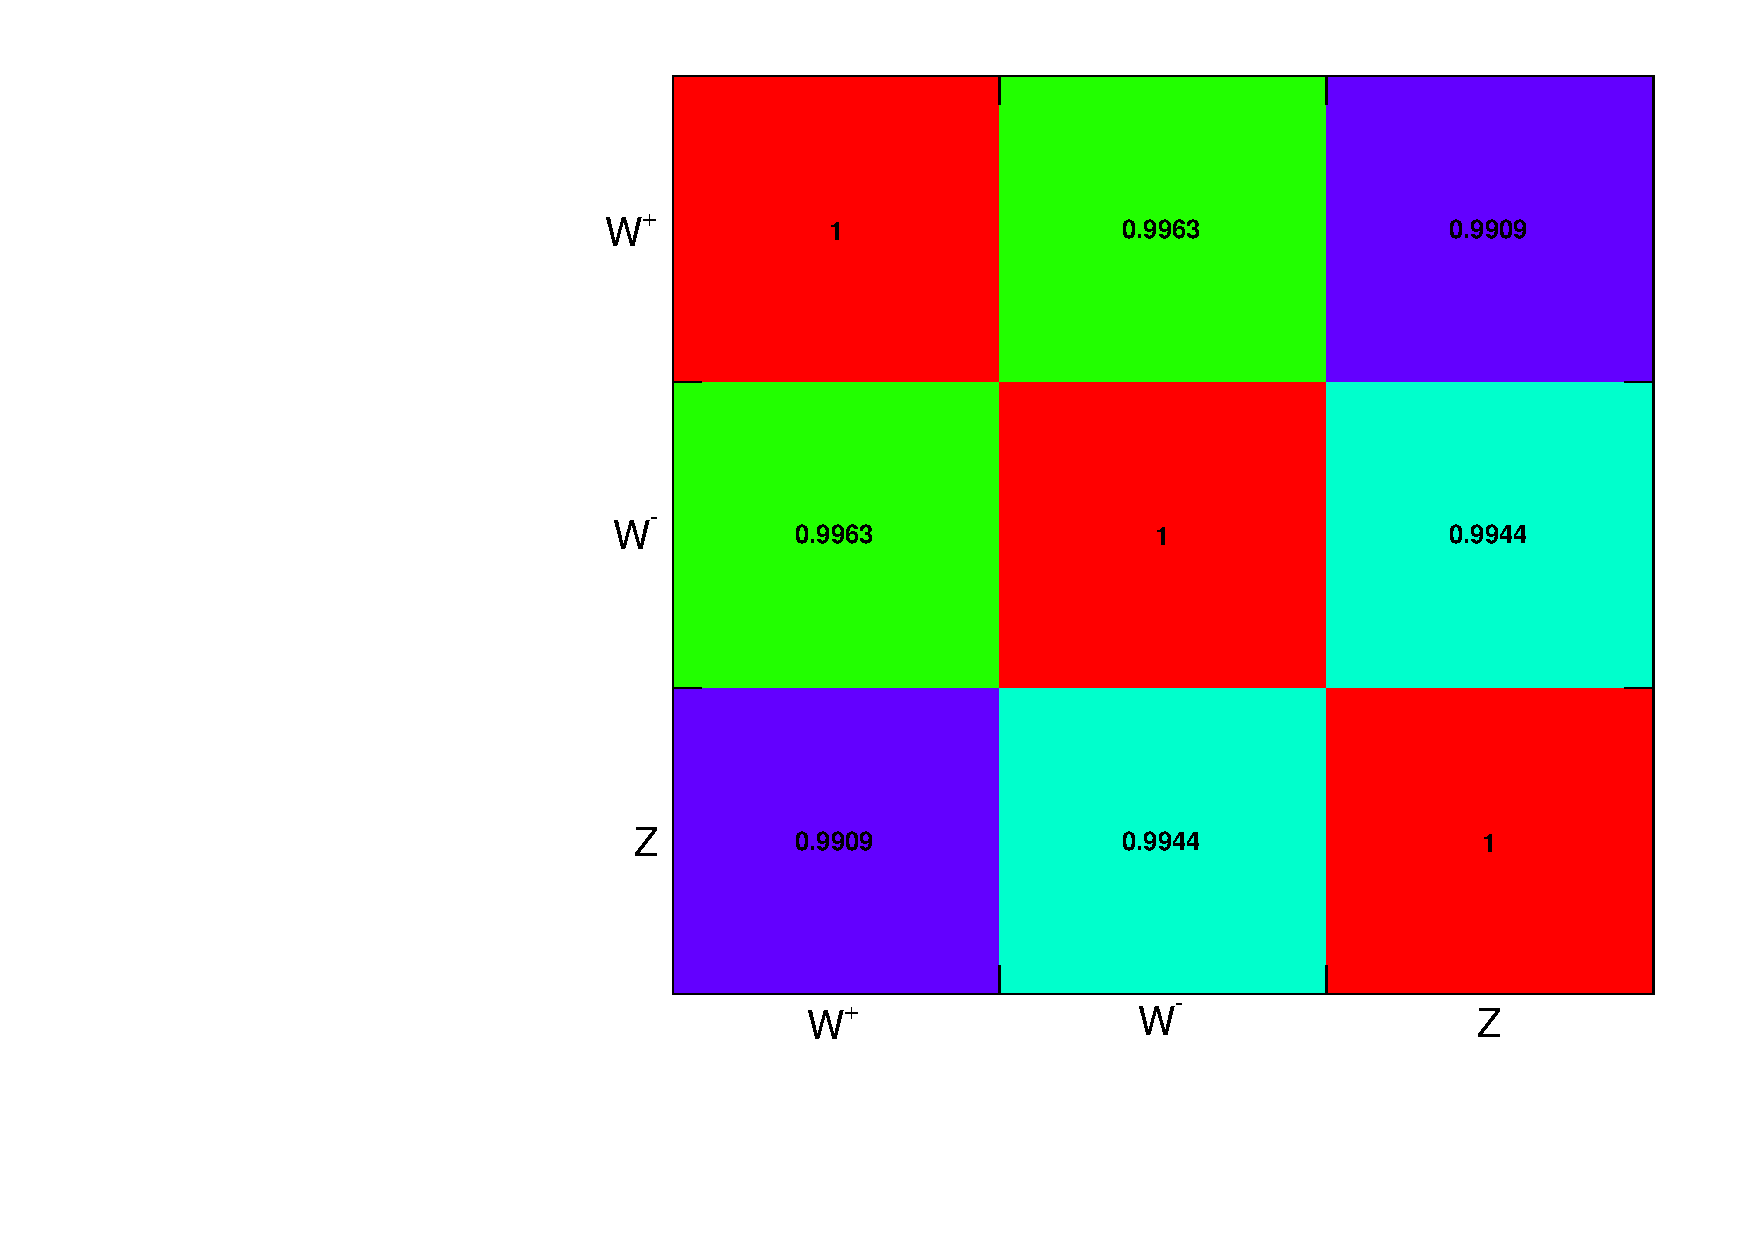
\includegraphics[width=1.0\linewidth]{Systematics/RecEff.pdf}  \\ a)}
\end{minipage}
\hfill
\begin{minipage}[h]{0.49\linewidth}
\center{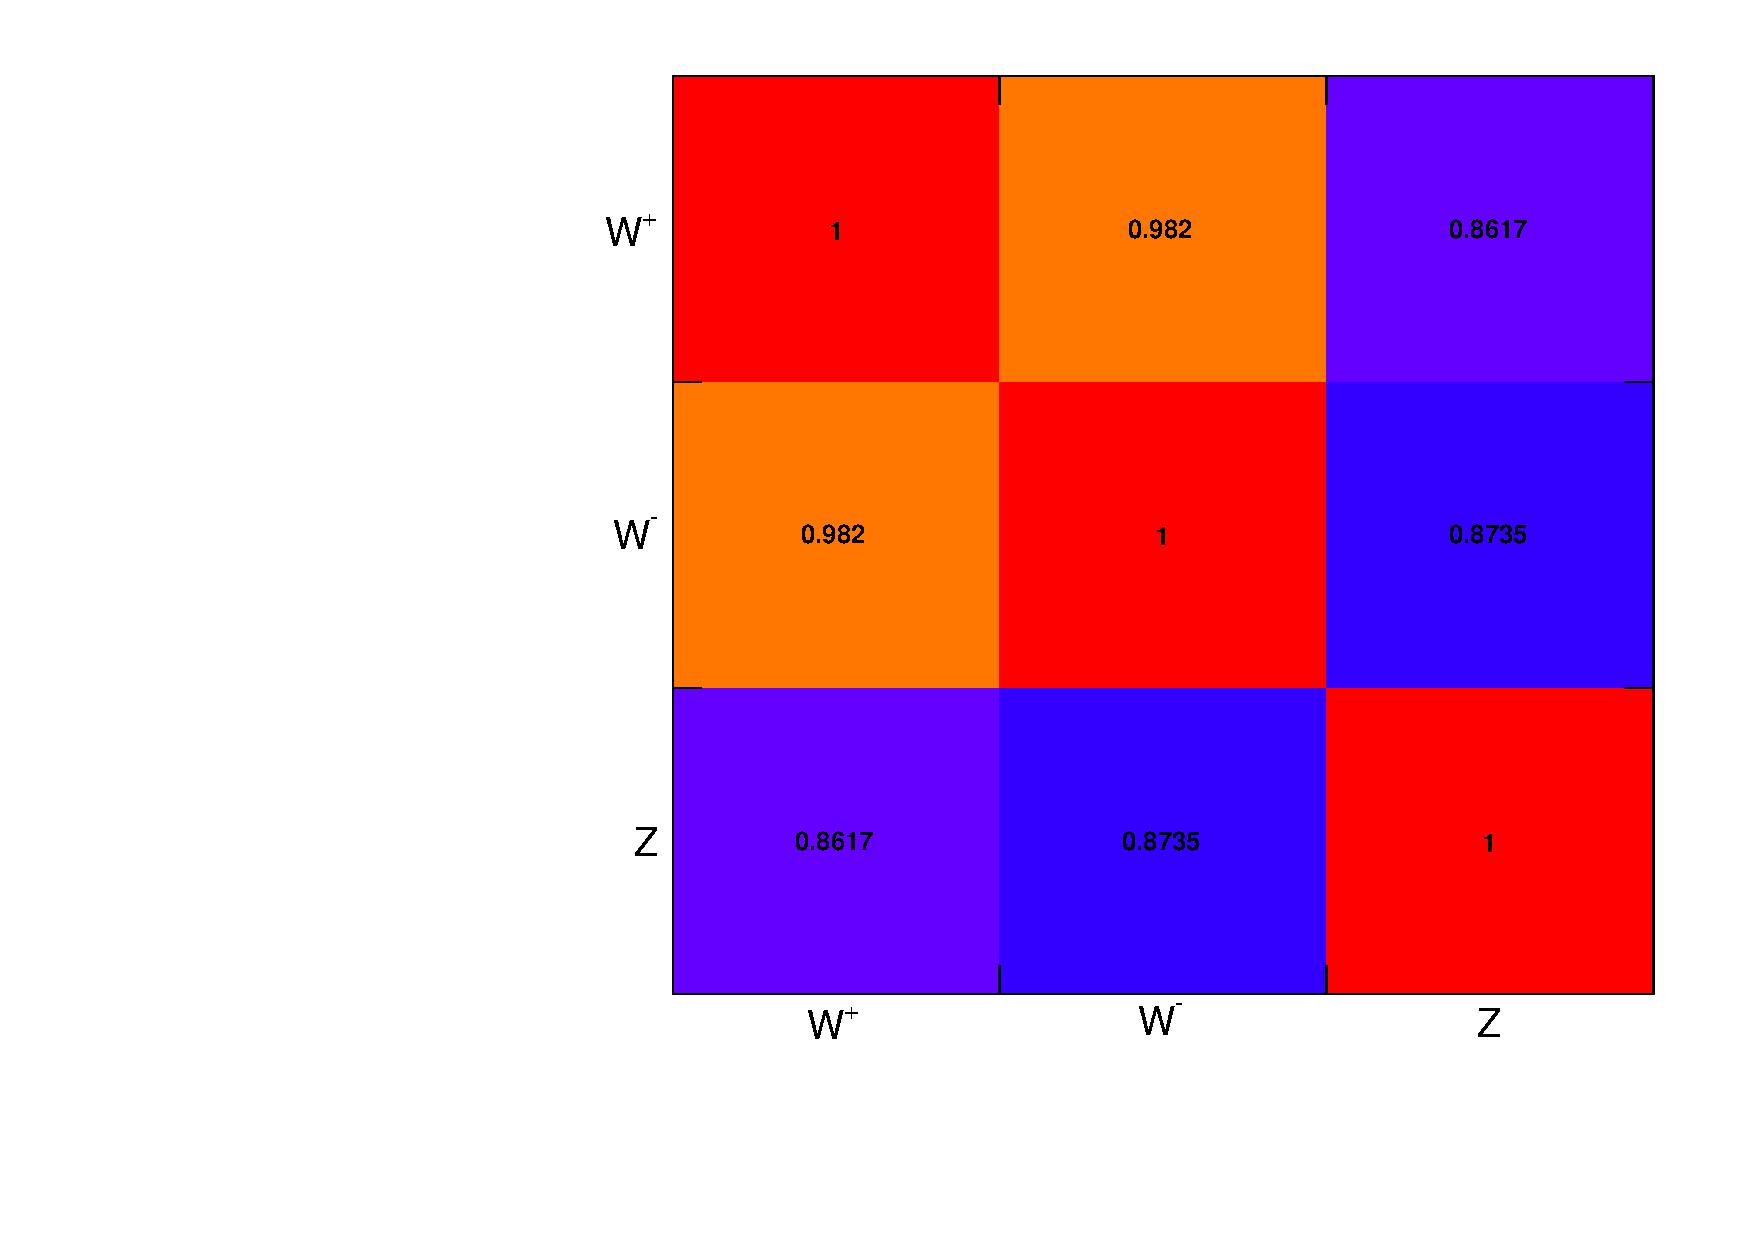
\includegraphics[width=1.0\linewidth]{Systematics/IDEff.pdf} \\ b)}
\end{minipage}
\vfill
\begin{minipage}[h]{0.49\linewidth}
\center{\includegraphics[width=1.0\linewidth]{Systematics/Trig.pdf}  \\ c)}
\end{minipage}
\hfill
\begin{minipage}[h]{0.49\linewidth}
\center{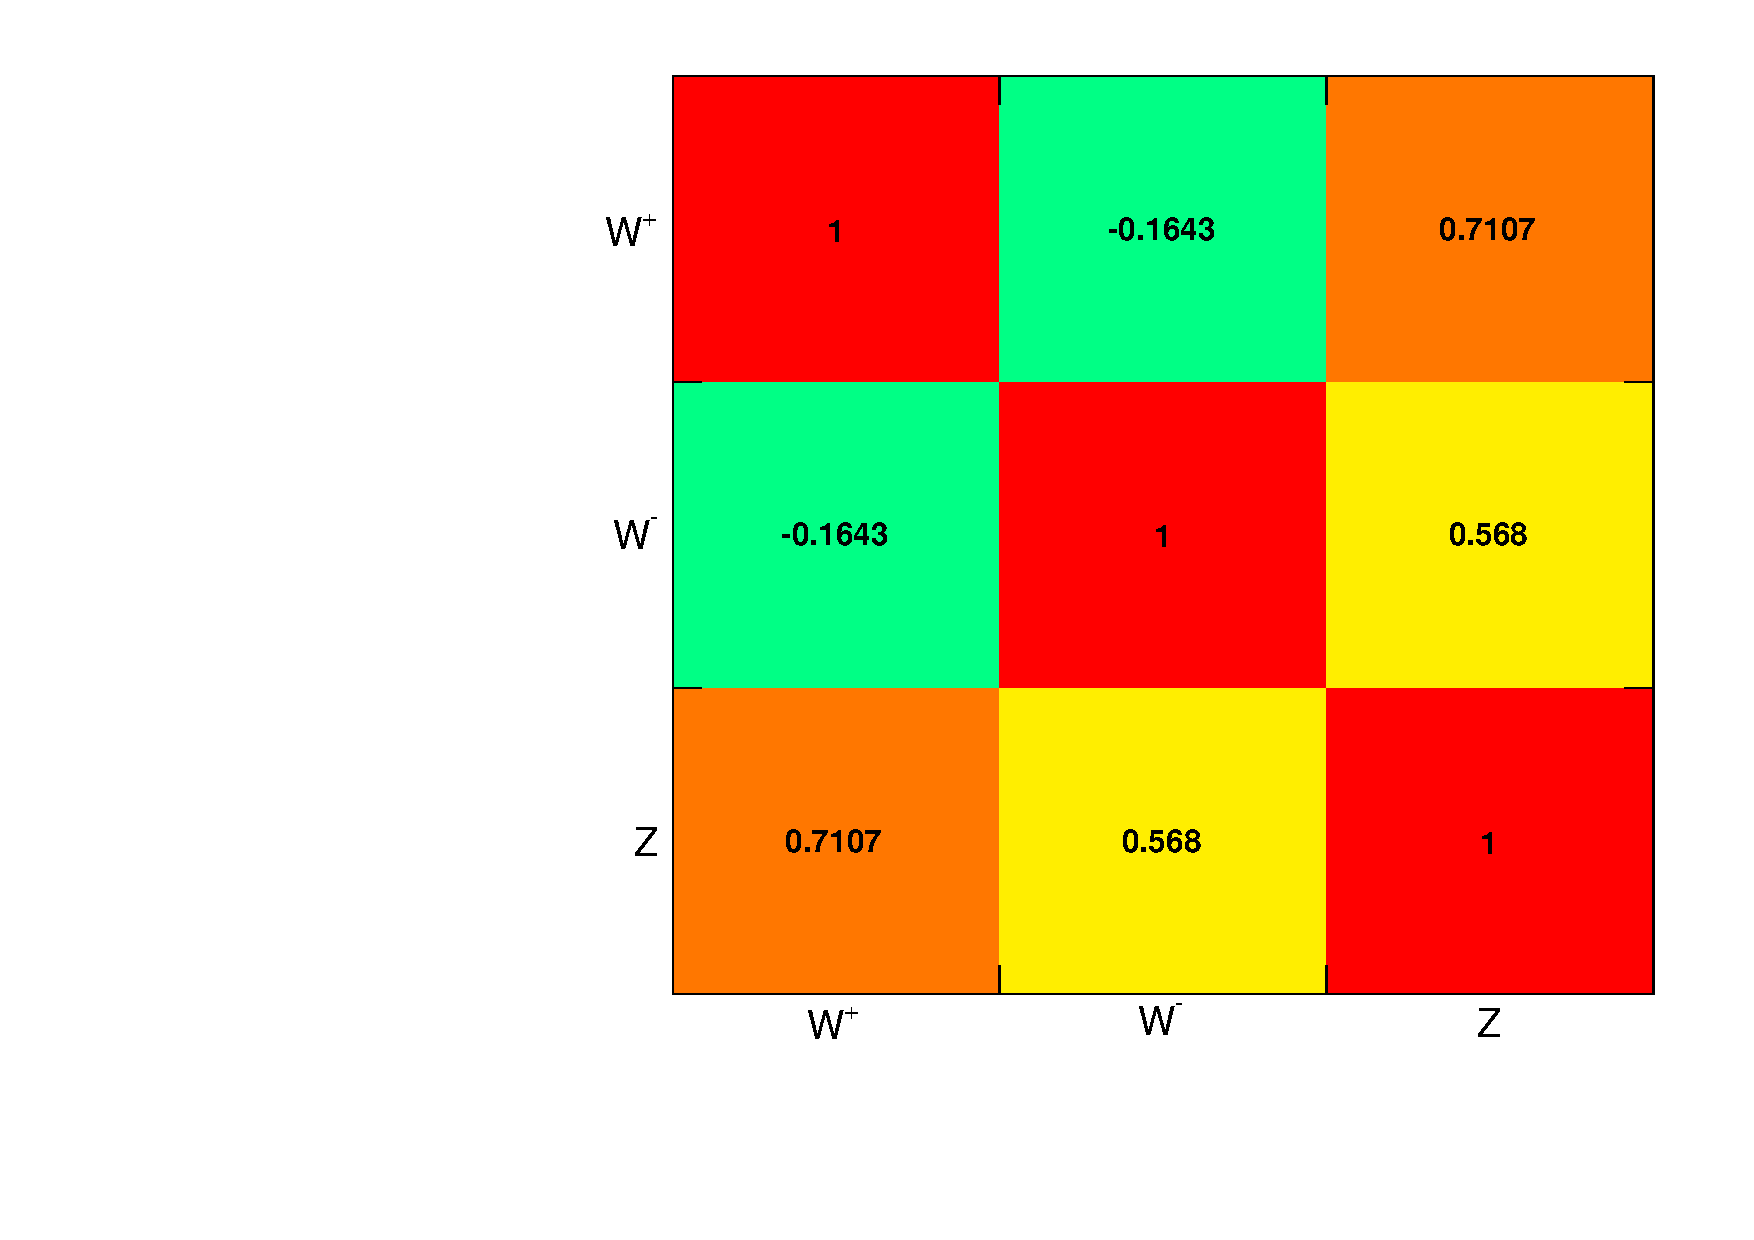
\includegraphics[width=1.0\linewidth]{Systematics/muIDEff.pdf} \\ d)}
\end{minipage}

\caption{Correlation coefficients $\rho_{XY}$ among $C_{Z}$ , $C_{W^{+}}$ and $C_{W^{-}}$   for a) electron reconstruction, b) electron identification, c) electron trigger and d) muon trigger scale factor uncertainties.}
\label{fig:CorToy}
\end{figure}

%\begin{minipage}[h]{0.43\linewidth}
%\center{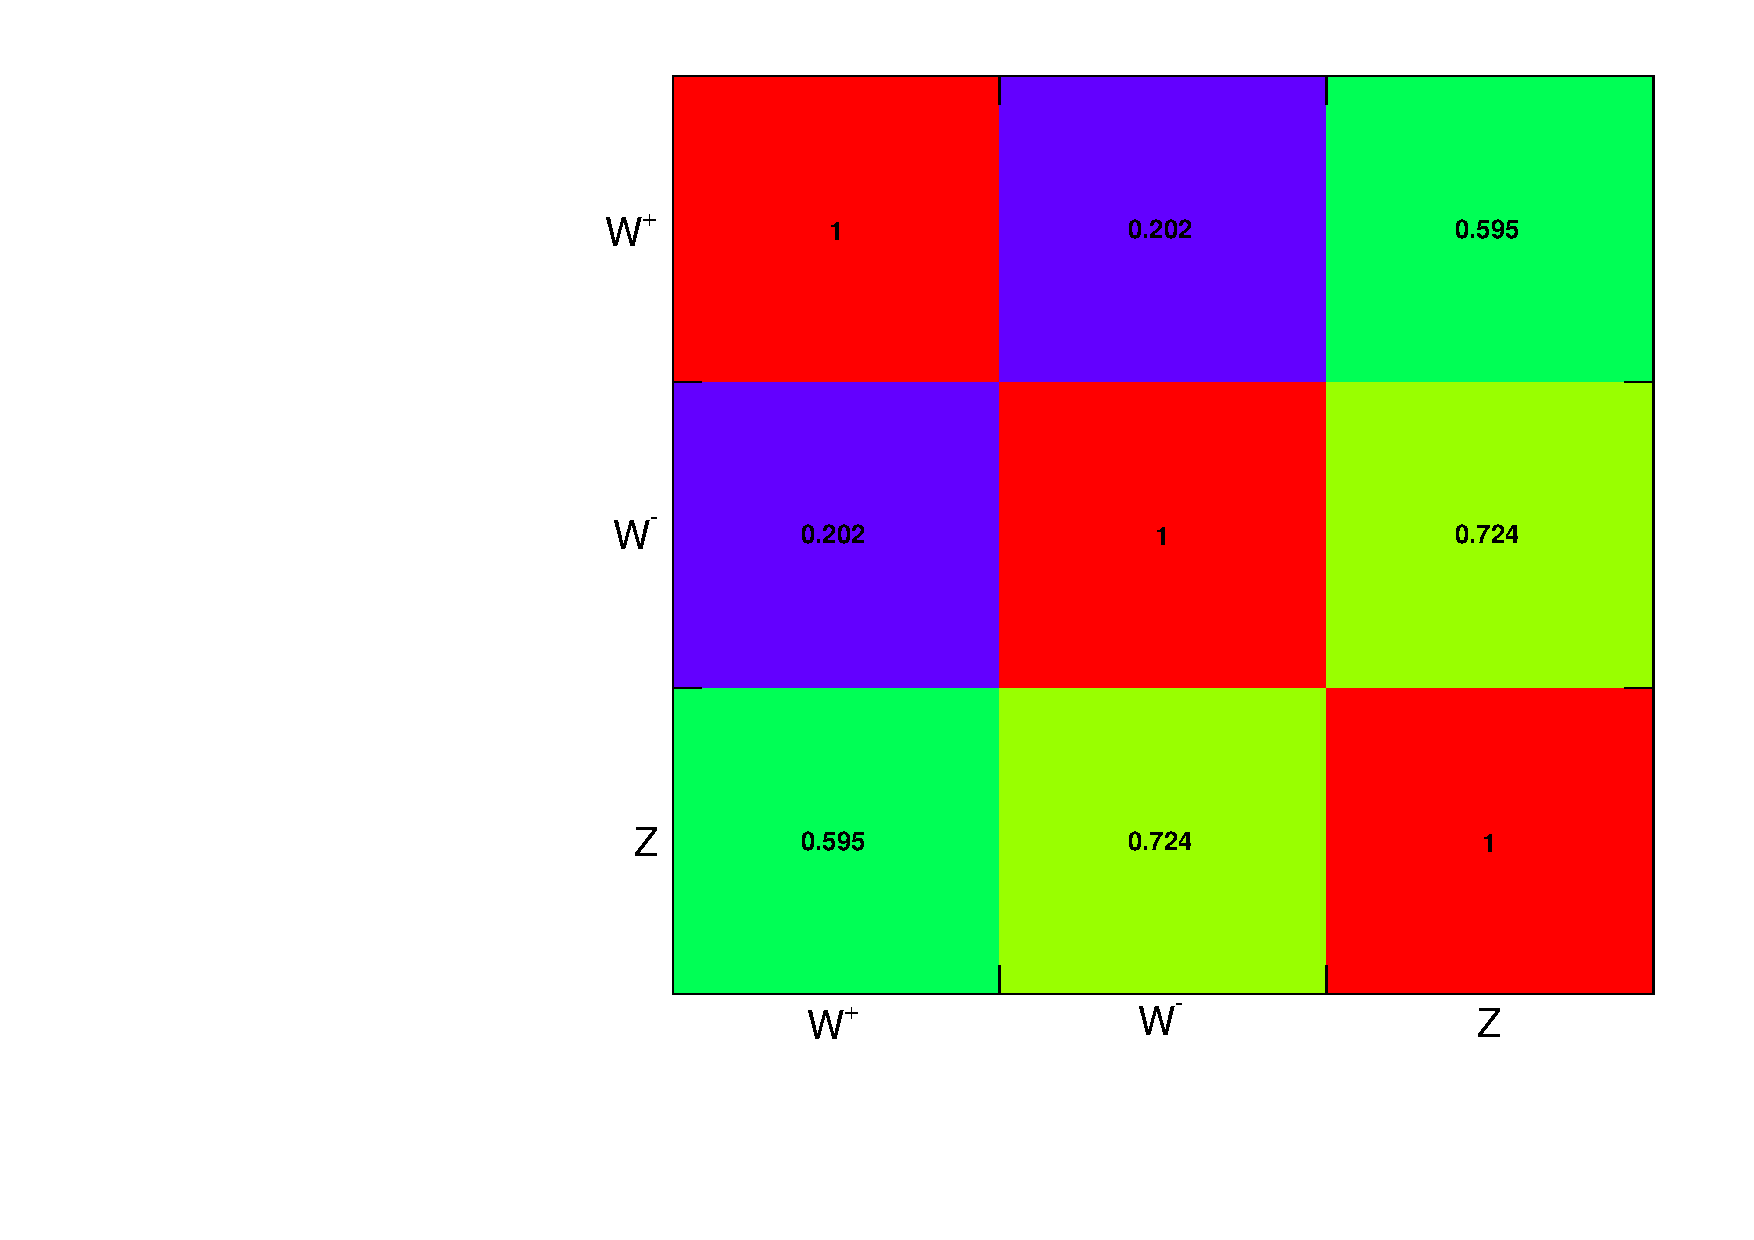
\includegraphics[width=1.0\linewidth]{Systematics/ePDFC.pdf}  \\ a)}
%\end{minipage}
%\hfill
%\begin{minipage}[h]{0.43\linewidth}
%\center{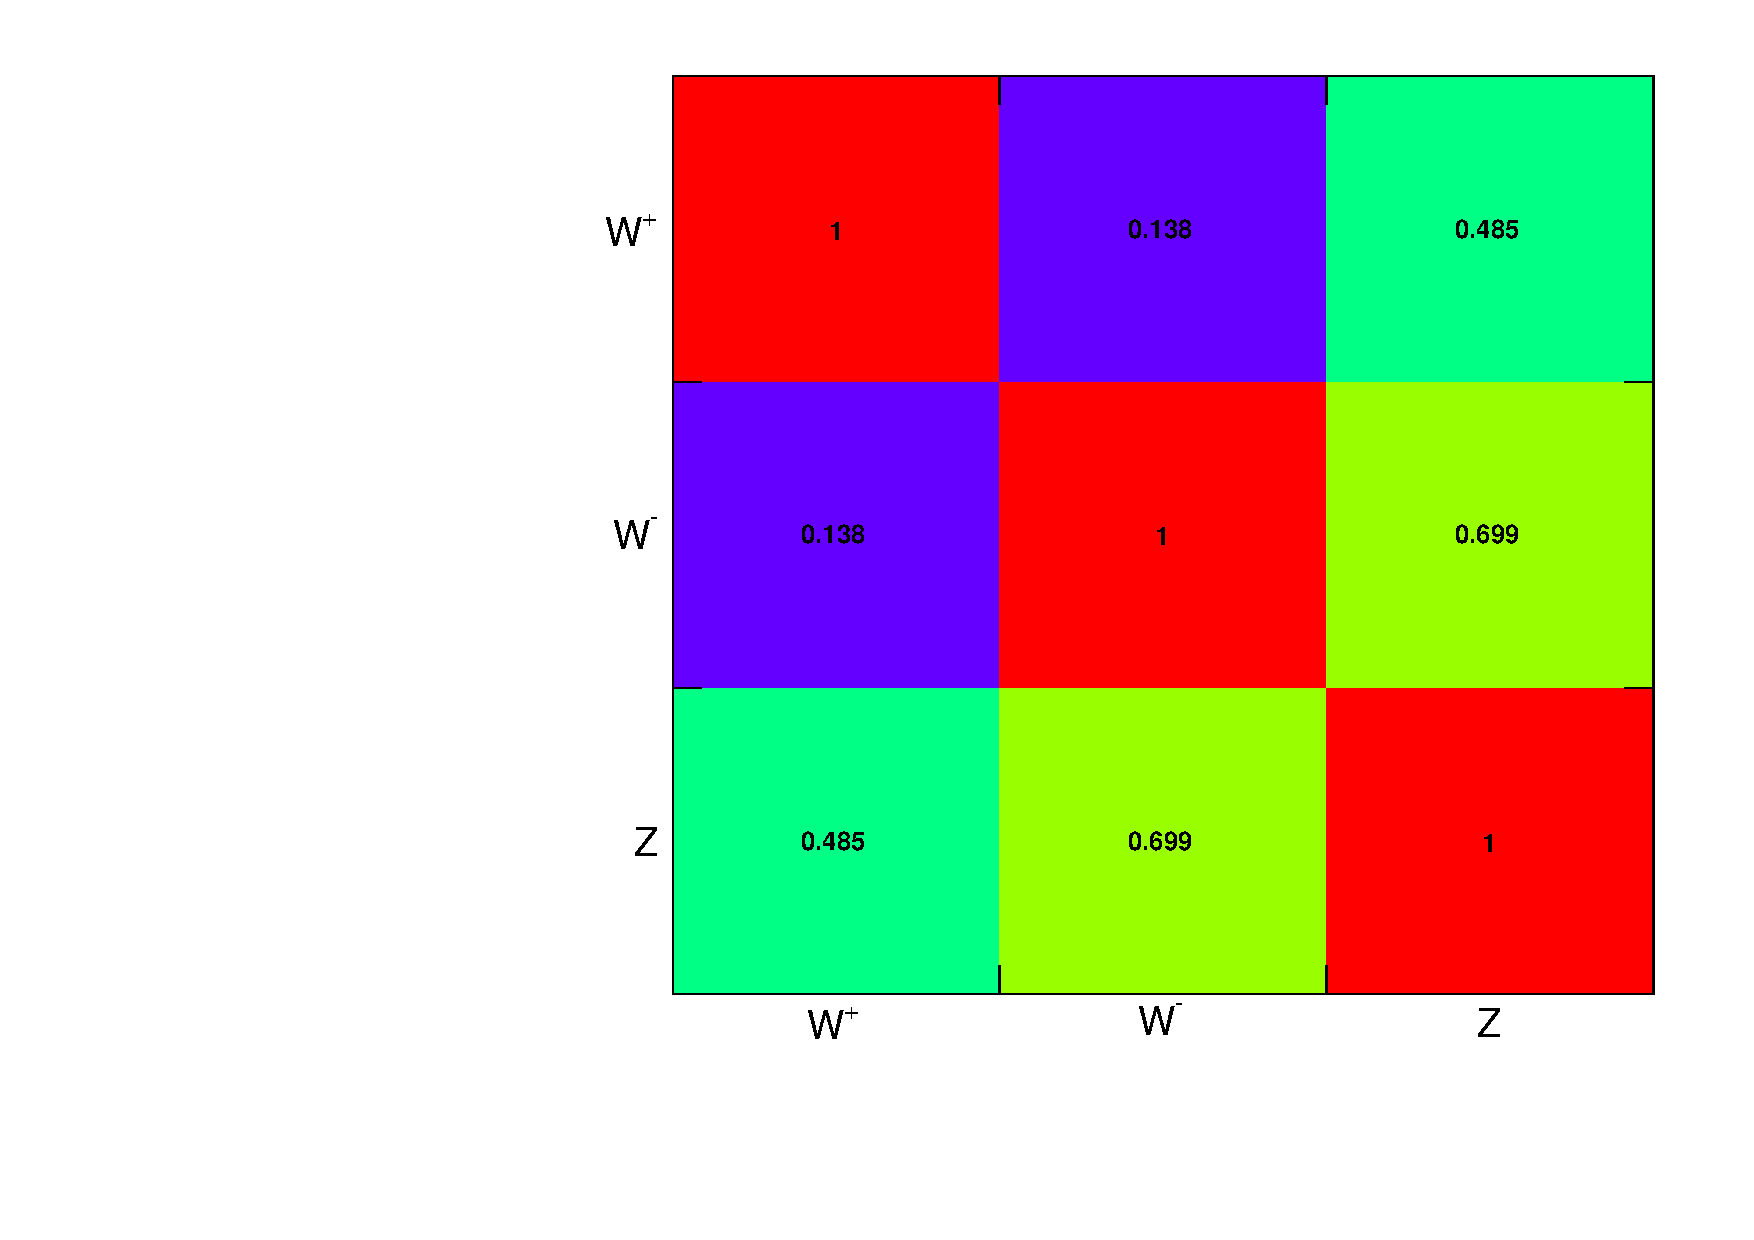
\includegraphics[width=1.0\linewidth]{Systematics/mPDFC.pdf} \\ b)}
%\end{minipage}
%\caption{Correlation coefficients $\rho_{XY}$ among $C_{Z}$ , $C_{W^{+}}$ and $C_{W^{-}}$  for the PDF uncertainty within 1 pdf set in a) electron and b) muon analyses.}
%\label{fig:ApdfErr}
%\end{figure}

\subsection{Treatment of partially correlated uncertainties}\label{sec:partCor}

The following uncertainties are considered to be partially correlated between $Z$, $W^{+}$ and $W^{-}$ analyses for an observables $o_X$ and $o_Y$:
\begin{itemize}
\item Electron trigger efficiency;
\item Electron resolution efficiency;
\item Electron identification efficiency;
\item Muon reconstruction and identification efficiency.
\end{itemize}

For each source of uncertainty a correlation coefficients between analysis X and Y can be estimated as:
\begin{equation}\label{eq:Corr}
\rho_{XY}=\frac{1}{\sigma(o_X)\sigma(o_Y)}\cdot \frac{1}{N} \sum_{i=1}^N (o^i_X-\bar{o}_X) (o^i_Y-\bar{o}_Y)=\frac{C_{XY}}{\sigma(o_X)\sigma(o_Y)},
\end{equation}
where $\bar{o}_X$ and $\bar{o}_Y$ are the mean values of $o_X$ and $o_Y$ respectively,  $\sigma(o_X)$ and $\sigma(o_Y)$ are the uncertainties and $i$ runs over the number of experiments N. $C_{XY}$ denotes elements of the covariance matrix. Resulting correlation matrices for each Toy MC systematic source are shown in Fig.~\ref{fig:CorToy}.


%Correlation coefficients for a systematic error within 1 pdf set are considered independent for each eigenvectors. Using the Eq.~\ref{eq:Corr} and~\ref{eq:PDF} the total correlation matrix $C^{PDF}_{XY}$ can be calculated as:
%\begin{equation}
%C^{PDF}_{XY}= \frac{1}{4}\sum(X^{+}-X^{-})\cdot (Y^{+}-Y^{-}).
%\end{equation}
%The resulting covariance matrix for an A factor is shown in Fig.~\ref{fig:ApdfErr}.

In order to include these covariances in further calculations, the Cholesky decomposition \cite{Dickinson1978} have been performed. Using it, the covariance matrix C is re-written as:
\begin{equation}
C=L \cdot L^{T},
\end{equation}
where $L$ is a lower triangular matrix, and $L^{T}$ is a transpose of L. This decomposition is always unique because the covariance matrix has a positive definitive.
 
Rows of the matrix L are corresponding to the three systematic error vectors, that are fully correlated between $W^{+}$, $W^{-}$ and $Z$ analyses. The quadratic sum of each row is corresponding to a total systematic uncertainty:
\begin{equation}
\sigma_{X}^{tot} = \sum_{i}^3 L_{iX}^2.
\end{equation}
The results of the Cholesky decomposition could be found in Appendix~\ref{app:Chol}.